%====================================================================
%====================================================================
\backupbegin 
\section*{Backup}
%====================================================================
\frame[allowframebreaks]{ \frametitle{References}
  {%\footnotesize
   \tiny
   \bibliography{/home/robin/Biblio/BibGene}
%    \bibliographystyle{/home/robin/LATEX/Biblio/astats}
   \bibliographystyle{alpha}
  }
}

%==================================================================
\frame{\frametitle{Latent network}

  \paragraph{Some undesirable property:} {all latent (GGM) models} infer the dependency struture of the latent $Z$, not of the observed abundances $Y$
  
  \bigskip \bigskip 
  \renewcommand{\nodesize}{2em}
  \begin{overprint}
    \onslide<2>
    $$
    \begin{array}{ccc}
    p(Z, Y) & & p(Y) \\ ~\\
      \begin{tikzpicture}[scale=.8]
  \node[hidden] (Z1) at ( 0.95*\edgeunit,  0.31*\edgeunit) {$Z_1$};
  \node[hidden] (Z2) at (-0.00*\edgeunit,  1.00*\edgeunit) {$Z_2$};
  \node[hidden] (Z3) at (-0.95*\edgeunit,  0.31*\edgeunit) {$Z_3$};
  \node[hidden] (Z4) at (-0.59*\edgeunit, -0.81*\edgeunit) {$Z_4$};
  \node[hidden] (Z5) at ( 0.59*\edgeunit, -0.81*\edgeunit) {$Z_5$};
  
  \draw[edge] (Z1) to (Z5);  \draw[edge] (Z2) to (Z3);  
  \draw[edge] (Z2) to (Z4);  \draw[edge] (Z3) to (Z4); 

  \node[observed] (Y1) at ( 1.05*\edgeunit, -0.39*\edgeunit) {$Y_1$};
  \node[observed] (Y2) at (-0.00*\edgeunit,  0.30*\edgeunit) {$Y_2$};
  \node[observed] (Y3) at (-1.05*\edgeunit, -0.39*\edgeunit) {$Y_3$};
  \node[observed] (Y4) at (-0.59*\edgeunit, -1.51*\edgeunit) {$Y_4$};
  \node[observed] (Y5) at ( 0.59*\edgeunit, -1.51*\edgeunit) {$Y_5$};
  
  \draw[arrow] (Z1) to (Y1); 
  \draw[arrow] (Z2) to (Y2);
  \draw[arrow] (Z3) to (Y3);
  \draw[arrow] (Z4) to (Y4);
  \draw[arrow] (Z5) to (Y5);
  \end{tikzpicture}

    & \qquad \qquad &
      \begin{tikzpicture}[scale=.8]
  \node[observed] (Y1) at ( 0.95*\edgeunit,  0.31*\edgeunit) {$Y_1$};
  \node[observed] (Y2) at (-0.00*\edgeunit,  1.00*\edgeunit) {$Y_2$};
  \node[observed] (Y3) at (-0.95*\edgeunit,  0.31*\edgeunit) {$Y_3$};
  \node[observed] (Y4) at (-0.59*\edgeunit, -0.81*\edgeunit) {$Y_4$};
  \node[observed] (Y5) at ( 0.59*\edgeunit, -0.81*\edgeunit) {$Y_5$};
  \node[empty] (YY) at ( 0.59*\edgeunit, -1.51*\edgeunit) {};

  \draw[edge] (Y1) to (Y5);  \draw[edge] (Y2) to (Y3);  
  \draw[edge] (Y2) to (Y4);  \draw[edge] (Y3) to (Y4);  
  
  \end{tikzpicture}

    \end{array}
    $$
    \onslide<3>
    $$
    \begin{array}{ccc}
    p(Z, Y) & & p(Y) \\ ~\\
      \begin{tikzpicture}[scale=.8]
    \node[hidden] (Z1) at ( 0.95*\edgeunit,  0.31*\edgeunit) {$Z_1$};
    \node[hidden] (Z2) at (-0.00*\edgeunit,  1.00*\edgeunit) {$Z_2$};
    \node[hidden] (Z3) at (-0.95*\edgeunit,  0.31*\edgeunit) {$Z_3$};
    \node[hidden] (Z4) at (-0.59*\edgeunit, -0.81*\edgeunit) {$Z_4$};
    \node[hidden] (Z5) at ( 0.59*\edgeunit, -0.81*\edgeunit) {$Z_5$};
    
    \draw[edge] (Z1) to (Z2);  \draw[edge] (Z1) to (Z4);  
    \draw[edge] (Z1) to (Z5);  \draw[edge] (Z2) to (Z3);  
    \draw[edge] (Z2) to (Z4);  \draw[edge] (Z3) to (Z4); 

    \node[observed] (Y1) at ( 1.05*\edgeunit, -0.39*\edgeunit) {$Y_1$};
    \node[observed] (Y2) at (-0.00*\edgeunit,  0.30*\edgeunit) {$Y_2$};
    \node[observed] (Y3) at (-1.05*\edgeunit, -0.39*\edgeunit) {$Y_3$};
    \node[observed] (Y4) at (-0.59*\edgeunit, -1.51*\edgeunit) {$Y_4$};
    \node[observed] (Y5) at ( 0.59*\edgeunit, -1.51*\edgeunit) {$Y_5$};

    \draw[arrow] (Z1) to (Y1); 
    \draw[arrow] (Z2) to (Y2);
    \draw[arrow] (Z3) to (Y3);
    \draw[arrow] (Z4) to (Y4);
    \draw[arrow] (Z5) to (Y5);
  \end{tikzpicture}

    & \qquad \qquad &
      \begin{tikzpicture}[scale=.8]
  \node[observed] (Y1) at ( 0.95*\edgeunit,  0.31*\edgeunit) {$Y_1$};
  \node[observed] (Y2) at (-0.00*\edgeunit,  1.00*\edgeunit) {$Y_2$};
  \node[observed] (Y3) at (-0.95*\edgeunit,  0.31*\edgeunit) {$Y_3$};
  \node[observed] (Y4) at (-0.59*\edgeunit, -0.81*\edgeunit) {$Y_4$};
  \node[observed] (Y5) at ( 0.59*\edgeunit, -0.81*\edgeunit) {$Y_5$};
  \node[empty] (YY) at ( 0.59*\edgeunit, -1.51*\edgeunit) {};

  \draw[edge] (Y1) to (Y2);  \draw[edge] (Y1) to (Y3);  
  \draw[edge] (Y1) to (Y4);  \draw[edge] (Y1) to (Y5);  
  \draw[edge] (Y2) to (Y3);  \draw[edge] (Y2) to (Y4); 
  \draw[edge] (Y2) to (Y5);  \draw[edge] (Y3) to (Y4);  
  \draw[edge] (Y3) to (Y5);  \draw[edge] (Y4) to (Y5);  
  \end{tikzpicture}

    \end{array}
    $$
  \end{overprint}
  \renewcommand{\nodesize}{\commonnodesize}
}

%====================================================================
\frame{\frametitle{Models for species interaction networks} 

  \begin{tabular}{cc}
    \hspace{-.04\textwidth}
    \begin{tabular}{p{.5\textwidth}}
      \paragraph{Tree species interactions \refer{VPD08}:} 
      \begin{itemize}
       \item $n = 51$ tree species
       \item $Y_{ij} =$ number of fungal parasites shared by species $i$ and $j$
       \item $x_{ij} =$ vector of similarities (taxonomic, geographic, genetic) between species $i$ and $j$
      \end{itemize}
      
      \bigskip \bigskip
      \paragraph{Questions:} 
      \begin{itemize}
       \item Is the network 'organized' in some way? \\~
       \item Do the covariate contribute to explain why species interact?
      \end{itemize}

      
%       \bigskip \bigskip 
%       \paragraph{Other types of network.} 
%       \begin{itemize}
%       \item plant-pollinator: mutualistic network (bipartite) 
%       \item predator-prey: trophic network (multipartite)
%       \end{itemize}
    \end{tabular}
    &
    \begin{tabular}{p{.45\textwidth}}
      \paragraph{Network (weighted):} \\
%       \includegraphics[height=.25\textwidth,width=.25\textwidth,trim=30 30 30 30]     
      \includegraphics[height=.3\textwidth,width=.3\textwidth]{\fignet/Tree-netCircle}
 \\
      \paragraph{Adjacency matrix (counts):} \\
      \includegraphics[height=.3\textwidth,width=.3\textwidth]{\fignet/Tree-adjMat}
    \end{tabular}
  \end{tabular}
      
}

%====================================================================
\frame{\frametitle{PLN for dimension reduction (PCA)}

  \begin{tabular}{cl}
    \hspace{-.04\textwidth}
    \begin{tabular}{p{.3\textwidth}}
      \paragraph{Metabarcoding data} \refer{JFS16} \\ ~
      \begin{itemize}
      \item $p = 114$ OTUs (bacteria and fungi) \\ ~
      \item $n = 116$ leaves \\ ~
      \item collected on 3 trees 
        \begin{itemize}
        \item resistant 
        \item intermediate
        \item susceptible       
      \end{itemize}
      to oak powdery mildew
      \end{itemize}

      \bigskip \bigskip 
      \paragraph{Model selection:} 
      \begin{itemize}
        \item Penalized lower-bound $J(\widehat{\theta}, \widehat{q})$ \\
        (pseudo BIC, pseudo ICL, \dots)
      \end{itemize}

    \end{tabular}
    &
    \begin{tabular}{p{.55\textwidth}}
    \includegraphics[height=.4\textheight]{\fignet/CMR18-AnnApplStat-Fig4a} \\
    ~ \\
    \includegraphics[height=.4\textheight]{\fignet/CMR18-AnnApplStat-Fig5a} 
    \end{tabular}
  \end{tabular}
}

%====================================================================
\frame{\frametitle{Poisson SBM with covariates: choosing $K$}

  \begin{tabular}{c|c|c}
    & & \paragraph{Including the} \\
    & \paragraph{No covariate} & \paragraph{taxonomic distance} \\
    & & \\
    Observed network & Clustering (no covariate) & Group composition \\
    \includegraphics[width=.3\textwidth]{\fignet/Tree-adjMat}
    &
    \includegraphics[width=.3\textwidth]{\fignet/Tree-adjMat-SBMnull}
    &
    \includegraphics[width=.3\textwidth]{\fignet/Tree-adjMat-SBMtaxo}
    \\
    Model selection & Clustering & Group composition \\
    \includegraphics[width=.3\textwidth,width=.25\textwidth]{\fignet/Tree-ICL-SBMall}
    &
    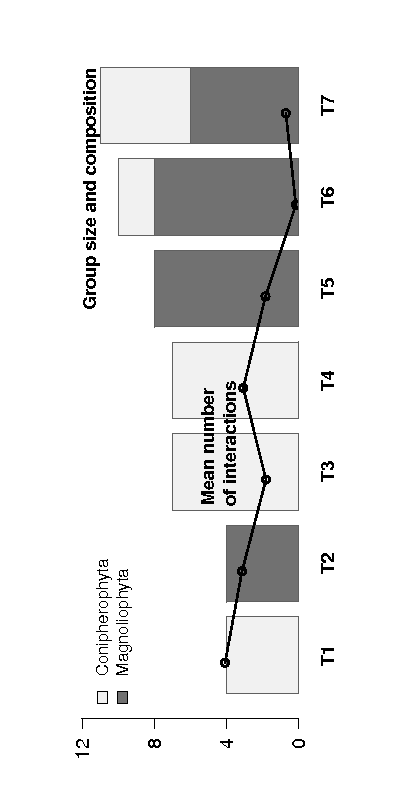
\includegraphics[width=.3\textwidth,height=.25\textwidth,trim=0 20 0 100]{\fignet/MRV10_AoAS_Q7_group}
    &
    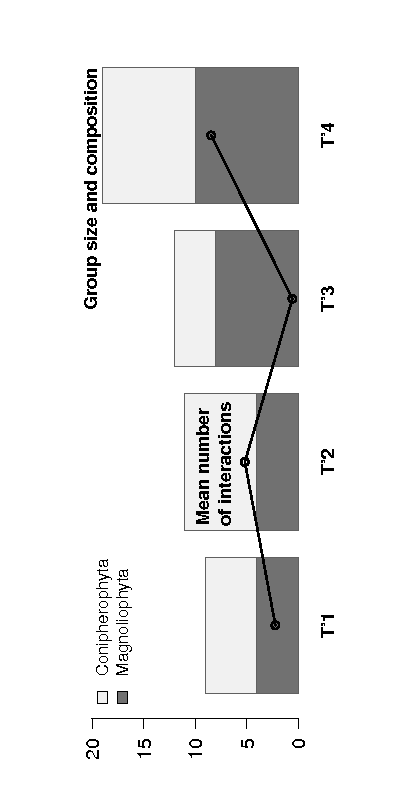
\includegraphics[width=.3\textwidth,height=.25\textwidth,trim=0 20 0 100]{\fignet/MRV10_AoAS_Q4_group}  
  \end{tabular}

}

%====================================================================
\frame{\frametitle{Tree interaction network: posterior distributions} 

  \bigskip 
  \paragraph{Do the distance between the tree species contribute to structure network?} \refer{DoR19}
  $$
  \begin{tabular}{ccc}
    taxonomy & geography & genetics \\
    \includegraphics[width=.25\textwidth]{\figbayes/Tree-all-V10-M5000-beta1} & 
    \includegraphics[width=.25\textwidth]{\figbayes/Tree-all-V10-M5000-beta2} & 
    \includegraphics[width=.25\textwidth]{\figbayes/Tree-all-V10-M5000-beta3}
  \end{tabular}
  $$
  
  \bigskip \pause
  \hspace{-.025\textwidth}
  \begin{tabular}{rrrr}
    \paragraph{Correlation between estimates.} 
    & $(\beta_1, \beta_2)$ & $(\beta_1, \beta_3)$ & $(\beta_2, \beta_3)$ \\
    $p_{VEM}(\beta)$    & $-0.012$ & $ 0.021$ & $ 0.318$ \\
    $p(\beta \mid Y)$ & $-0.274$ & $-0.079$ & $-0.088$
  \end{tabular}

  \bigskip \bigskip 
  \paragraph{Model selection.} 
  $$
  P\{X = \text{(taxo., geo.)} \mid Y \} \simeq 70\%, \qquad
  P\{X = \text{(taxo.)} \mid Y \} \simeq 30\%
  $$

}

%====================================================================
\frame{\frametitle{Fish species in the Barents sea}

  \newcommand{\figStR}{/home/robin/RECHERCHE/BAYES/PLNsampling/Paper/Figures}
  \newcommand{\nIterEx}{10000} \newcommand{\lagEx}{50} \newcommand{\nISex}{200}
  \newcommand{\exampleParms}{-nIter\nIterEx-lag\lagEx-nIS\nISex}
  \newcommand{\nIterSel}{\nIterEx} \newcommand{\lagSel}{20} \newcommand{\nISsel}{\nISex}
  \newcommand{\selectParms}{-nIS\nISsel-nIter\nIterSel-lag\lagSel}
  
  \bigskip
  \paragraph{Comparison of the estimates.} \refer{StR24}
  $$
  \begin{tabular}{ccc}
    $\widehat{B}$ & $\widehat{\Sigma}$ & ESS (CL5) \\
    \includegraphics[width=.25\textwidth, trim=10 10 25 50, clip=]{\figStR/Barents\exampleParms-compBeta-cem5-all} & 
    \includegraphics[width=.25\textwidth, trim=10 10 25 50, clip=]{\figStR/Barents\exampleParms-compSigma-cem5-all} & 
    \includegraphics[width=.25\textwidth, trim=10 10 25 50, clip=]{\figStR/Barents\exampleParms-ESS-cem5}     
  \end{tabular}
  $$

  \pause
  \paragraph{Significance.} Test statistics $\widehat{\theta} \left/ \sqrt{\widehat{\Var}_\infty(\widehat{\theta})} \right.$
  $$
  \begin{tabular}{ccc}
    $\widehat{B}$ & $\widehat{\Sigma}$ & $\text{cor}(\widehat{\Sigma})$ \\
    \includegraphics[width=.25\textwidth, trim=10 10 25 25, clip=]{\figStR/Barents\exampleParms-betaSignif-cem5} & 
    \includegraphics[width=.25\textwidth, trim=10 10 25 25, clip=]{\figStR/Barents\exampleParms-sigmaSignif-cem5} &
    \includegraphics[width=.25\textwidth, trim=10 10 25 25, clip=]{\figStR/Barents\exampleParms-corSigmaSignif-cem5}
  \end{tabular}  
  $$
}

%====================================================================
\backupend 
%====================================================================

